\section{Versuchsaufbau und Versuchsdurchführung}

\begin{flushleft}
    Der Versuchsaufbau sieht wie folgt aus.
    Es wird ein Echoskop, mit einer $1\,\unit{\mega\hertz}$, blau markierten, sowie einer $2\,\unit{\mega\hertz}$, rot markierten, Sonde benötigt.
    Der Kippschalter an dem Echoskop wird auf \textit{REFLEC.} gestellt.
    Verbunden ist das Echoskop mit einem Rechner, auf welchem das Programm A-Scan zum auswerten der Messwerte verwendet wird.
    Zudem wird ein Acrylblock benötigt, welcher verschiedene Größen, sowie verschieden weit von der Kante entfernte Löcher hat.
    Unter diesen Acrylblock werden Papiertücher gelegt und als Kontaktmittel wird Wasser benutzt.
    Ebenso wird eine Schieblehre zum vermessen des Acrylblocks benötigt.
    Die Einstellungen in dem Programm A-Scan sehen wie folgt aus.
    In der obigen Zeile werden die Einstellungen \textit{Depth} und \textit{Amp} gewählt. 
    Bei \textit{Sound Velocity} wird die Schallgeschwindigkeit eingegeben und als letztes um die Messung zu starten wird \textit{Start} gedrückt.
\end{flushleft}

\begin{figure}[H]
    \centering
    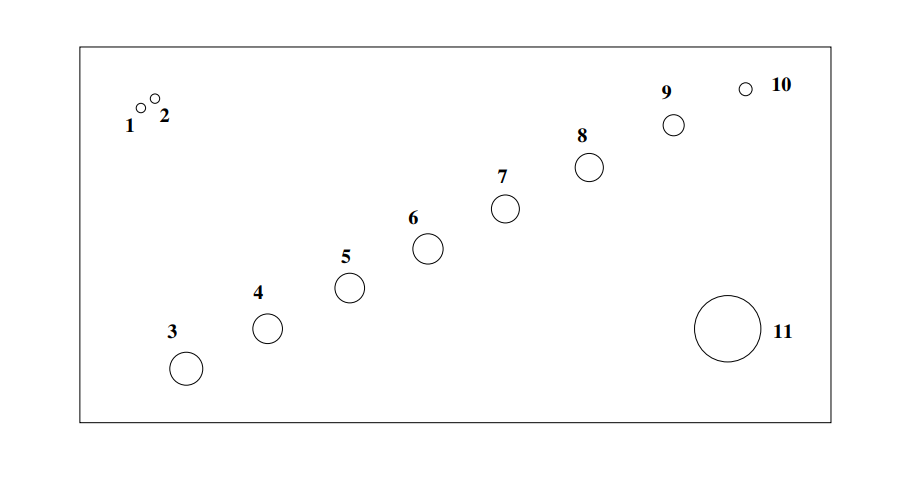
\includegraphics[height=60mm]{bilder/block.png}
    \caption{ Abbildung des Verwendeten Acrylblocks \label{Abbildung1}}
\end{figure}

\subsection{Untersuchung eines Acrylblocks mit dem A-Scan}

\begin{flushleft}
    Der Versuchs wird wie vorher beschrieben aufgebaut und der Acrylblock wird in Länge, Höhe und Tiefe mit der Schieblehre vermessen.
    Der Durchmesser der sieben zu vermessenden Löchern in dem Acrylblock werden ebenfalls gemessen.
    Danach wird die $2\,\unit{\mega\hertz}$ Sonde mit dem Kontaktmittel an der oberen Kante angelegt und die Messtiefe mit dem Programm A-Scan bestimmt.
    Die Messtiefe wird in $\unit{\micro\meter}$ angegeben und durch den herausstechenden Peak ermittelt.
    Nachdem die sieben Löcher von der einen Seite vermessen wurden, wird der Block um $180\unit{\degree}$ gedreht und die Messung erneut durchgeführt. 
\end{flushleft}

\subsection{Untersuchung des Auflösungsvermögen}

\begin{flushleft}
    Der Aufbau wird von dem vorherigen übernommen.
    Als nächstes werden diese zwei benachbarten Fehlstellen, oben links in Abbildung \ref{Abbildung1}, vermessen. 
    Dabei werden erst die $1\,\unit{\mega\hertz}$ Sonde und danach die $2\,\unit{\mega\hertz}$ Sonde verwendet.
    Die dabei entstehenden Bilder werden übernommen und es wird notiert was auffällt.
\end{flushleft}

\subsection{Untersuchung eines Acrylblocks mit dem B-Scan}

\begin{flushleft}
    Der Aufbau wird erneut übernommen, jedoch wird diesmal in der oberen Zeile die B-Scan Funktion ausgewählt.
    Damit werden die Löcher in dem Acrylblock erneut bestimmt, indem die Sonde ganz links auf der oberen Kante mit dem Kontaktmittel angesetzt wird und mit gleichmäßiger Geschwindigkeit nach ganz rechts bewegt.
    Durch das Bild, was dabei Erstellt wird, kann dann die Zeit sowie die Zeitdifferenz ermittelt und notiert werden.
\end{flushleft}

\subsection{Untersuchung eines Brustmodells mit einem B-Scan}

\begin{flushleft}
    Der Aufbau wird wieder übernommen und die B-Scan auf dem Rechner ausgewählt.
    Untersucht wird hierbei ein Brustmodell mit einer knotigen Anomalie. 
    Zuerst wird diese durch ertasten lokalisiert und danach mit der B-Scan Funktion des Brustmodells.
\end{flushleft}